% Author: Izaak Neutelings (November 2021)
\documentclass[border=3pt,tikz]{standalone}
\usepackage{amsmath} % for \text
\tikzset{>=latex} % for LaTeX arrow head

% colors
\colorlet{mylightred}{red!50!black!15}
\colorlet{mylightblue}{blue!50!black!15}
\colorlet{mylightgreen}{green!50!black!15}

\def\tick#1#2{\draw[thick] (#1) ++ (#2:0.02) --++ (#2-180:0.04)}

\begin{document}


% CONTROL REGIONS - with external plots
\def\s{6} % scale
\def\w{2.9} % figure width
\begin{tikzpicture}[x=\s cm,y=\s cm]
  
  % BOXES
  \fill [mylightred] % SR
    (0,0) rectangle (0.5,1);
  \fill [mylightgreen] % SB
    (0.5,0) rectangle (1,1);
  \draw[thick]
    (0,0) rectangle (1,1);
  
  % DASHED LINES
  \draw[dashed]
    (0.5,-0.06) -- (0.5,1);
  \draw[dashed]
    (0,0.5) -- (1,0.5);
  \tick{0,0}{0} node[left=1,scale=0.9] {0};
  \tick{0,0.5}{0} node[left=1,scale=0.9] {4};
  
  % AXIS LABELS
  \node[rotate=90,above] at (0,0.25) {``low''};
  \node[rotate=90,above] at (0,0.75) {``high''};
  \node[below] at (0.25,0) {3, ``low''};
  \node[below] at (0.75,0) {5--8, ``high''};
  \node[rotate=90,above=14] at (0,0.5) {HF activity [GeV]};
  \node[below=12] at (0.5,0) {Number of charge tracks $N_\text{ch}$};
  
  % FIGURES
  % control_region_plots_inputA.png is just a placeholder
  % here you can load plots as external figures to illustrate the ABCD method
  \node (A) at (0.75,0.75) {
    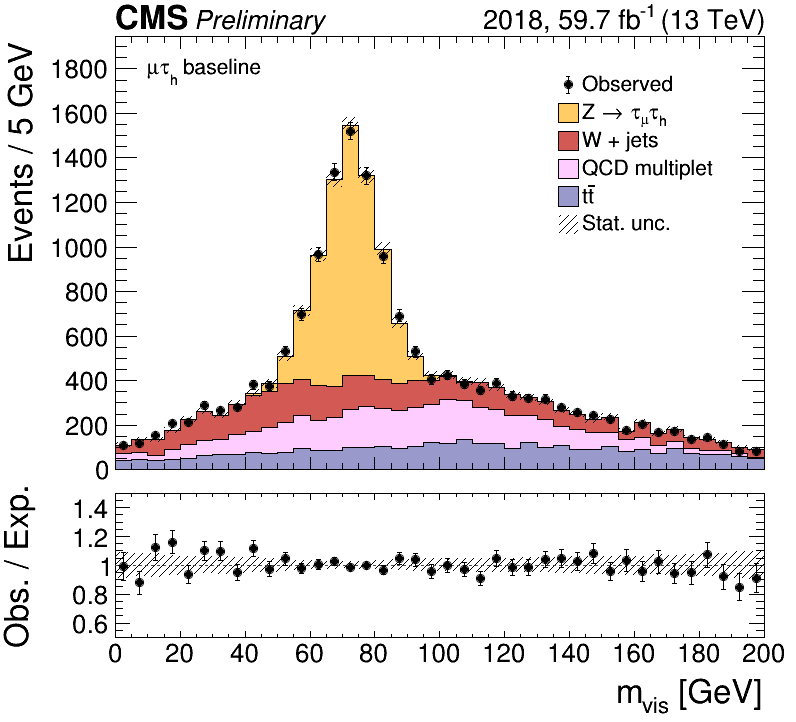
\includegraphics[width=\w cm,height=\w cm]{control_region_plots_A.png}};
  \node (B) at (0.25,0.75) {
    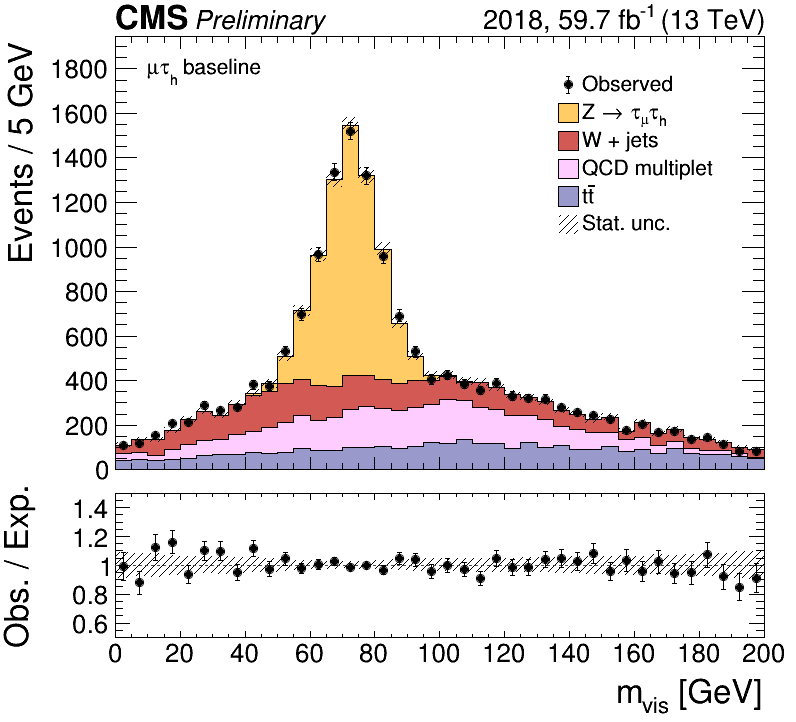
\includegraphics[width=\w cm,height=\w cm]{control_region_plots_A.png}};
  \node (C) at (0.75,0.25) {
    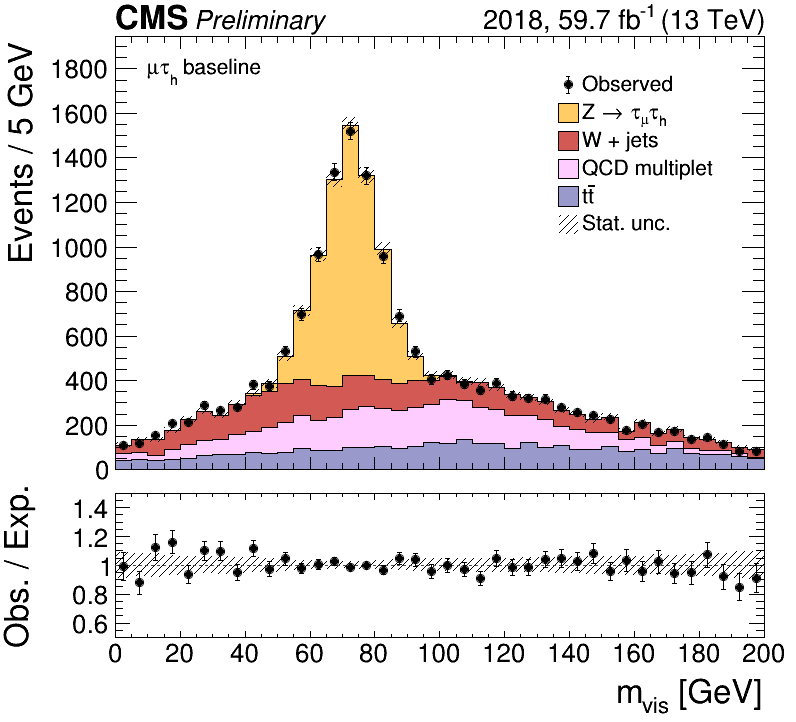
\includegraphics[width=\w cm,height=\w cm]{control_region_plots_A.png}};
  \node (D) at (0.25,0.25) {
    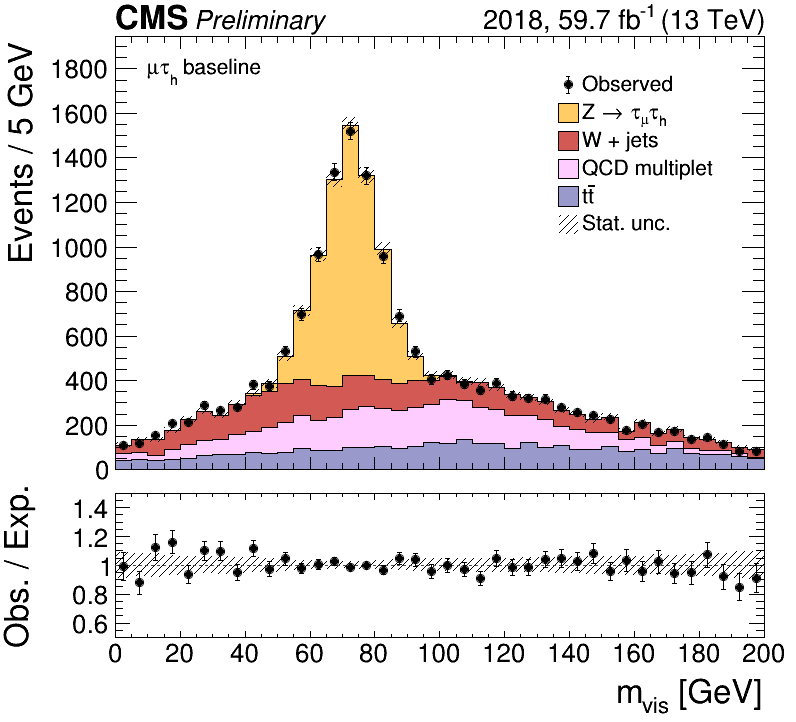
\includegraphics[width=\w cm,height=\w cm]{control_region_plots_A.png}};
    
  % REGION LABELS
  \node[above=7] (A) at (0.75,0.75) {A};
  \node[above=7] (B) at (0.25,0.75) {B};
  \node[above=7] (C) at (0.75,0.25) {C};
  \node[right=2,above=1,align=center]
    (D) at (0.25,0.25) {D\\[-2]\small signal region};
  
\end{tikzpicture}


\end{document}